



\chapter{Birth death catastrope -- Definition and main results}





\section{Chapter introduction}











We aim to understand the stochastics of those infections which exploit a lytic mechanism in their initial pathogenesis. That is to say, infectious agents which utilize intracellular environments to their proliferative advantage.\par

The importance of stochasticity can not be understated, because during the initial handful of replicative cycles, there is an exaggerated 
chance of an infection dying out before it gets started. Were we to use deterministic modeling, this perilous beginning is at risk of being glossed over with variable bacterial counts venturing between 1 and 0. \par

Hence, to really grasp the significance of \textit{why} Y. pestis, and other pathogens do what they do, we must account for the interplay of chance and fortune. 

It is for this reason we have selected the birth death catastrophe process as a tool of inquiry. \par
\vspace{25pt}




\noindent
Study of the birth death catastrophe (BDC) process and its dynamics will form a central focus of this thesis. Here
we present a series of results and analysis associated with its behaviour. As a continuois-time discrete-state Markov chain, 
the BDC process found its origin in a paper by Brokwell et. al. published 1982. During the late 1970s and early 80s,
attempts were being made to describe unpredictable population collapses using stochastic process theory:
\begin{quotation}
    "There has recently been a great deal of interest in the development and
    analysis of stochastic models for the growth of populations which are subject to
    catastrophes due either to death or large-scale emigrations" (Brockwell et. al. 1982)
\end{quotation}
Prior to that work models had largely incorporated deterministic growth interspersed by stochastic reductions --- sudden
drops, the sizes and times of which defined in distribution (Pakes et. al 1979). These suffered from peculiarities of 
modelling discrete populations with continuous random variables, and so attempts were made to to employ a step process; 
continuous time Markov chains in discrete state space.\par

Actually, the model presented in this 1982 paper is a generalisation of what we refer to as the BDC process. Not only
did it also include immigration events --- single steps-up occuring as a Poisson process with constant rate --- but also, the
catastrophic steps down in population count were sized as random i.i.d variables, with a few basic distributions investigated.
In our case, the catastrophe event is taken to reduce the population directly to 0, or to a special post catastrophe state,
$H$; in either case causing fixation.


Our interest in the Birth Death Catastrophe process stems from an application from within-host infection modelling. Like others before, we were interested in the pathogenesis behaviour of intracellular replication and bursting. Our agent of focus, Y. Pestis,
finds its way into host macrophaegs and replicates there, before ultimately lysing the cell so that the population of
infectious bacteria can traverse the extracellular matrix and continue their exploitative fight for survival.
"Catastrophe" here terms the cell-bursting event, which becomes increasingly likely as the intracellular population expands. 
Jonathan Carrthurs worked on the same model with focus on the agent Francisella Tularensis \cite{carruthers2020stochastic} \cite{karlin1957classification} \cite{karlin1982linear} \cite{di2008note}
, and similar work has
been directed towards the pathogenesis of salmonella.\par
My area of interest has been the potential importance of this replication and bursting strategy, along with other particular
behaviours of Y. Pestis, for an advantage in early pathogenesis --- getting a foothold when numbers are few, before a
serious immune response arives. This will be explored in chapter 3, but for the purposes of this present chapter, we will take the Birth Death Catastrophe process
as an abstract model, unbound by specific application. Here we will present a number of mathematical results which
quantify the stochastics of its growth and fixation over time.\par
\vspace{5pt}



\subsubsection*{Further interest}
Interest in the dynamics of catastrophic population decline is nothing new. Towards the end of the 18th century, 
Thomas Malthus published his fears of impending societal collapse. He worried that a geometrically growing
census would be less and less supported by only arithmetic development in food production, ultimately resulting in mass
famines. In the relevant literature, such population reductions by external factors are termed "positive checks".
This is as opposed to "preventative checks" by which individuals have fewer children to account for resource scarcity.

In 1755, Just 11 years before Thomas Malthus was born, Lisbon experienced a substantial earthquake devastating the city.
Voltaire includes a graphic scene of this in his allegorical novel, Candide. Perhaps catastrophe was on the mind of the time.
And maybe anxiety was justified. France, after all, was on the brink of revolution: 

\begin{quotation}
"War had created such social systems of unprecedented complexity that they exceeded the capacities of their internal
regulatory mechanisms to orchestrate the behavious of their parts. When, as in France, administrative chaos became too 
great and the government collapsed --- an event easily measured by the financial crisis of 1788 --- society exploded." (Artigiani, 1987) \cite{artigiani1987revolution}
\end{quotation}    

% "In the resulting conflagration, a phase change occurred that produced a non-linear social transformation, leaving in its 
% wake not only a new, simpler governmental structure but also a populance with new values. New values ensured that behaviour was more 
% attuned to the environment altered by previous developments. The new structure was more homogeneous than the ancien regime"

This quote is from a paper which attempts to apply Prigogine's theory of dissipative structures in understanding the 
evolution of culture and societal norms through revolutions. It's perhaps ambitious, and lacking in empirical merit.
But yet I quite like it. And similarly, I am curious of the prospect that the BDC process, or a variant of it, can be taken 
in allegory to illustrate a general behaviour observed in dissipative structures present accross multiple dynamic
phenomena. This will be explored further in chapter 4.\par 

I have also been interested in the role of catastrophic events in triggering evolutionary transitions. A notable example
is the KT boundary, where 65 million years ago much of life on earth was wiped out by an astroid. This set the stage for a 
mass proliferation and diversification of mammels.\par

It has also been postulated that the catastrophes of plague in Europe and their aftermath contributed 
to advancements in technology and culture. Most recently by James Belich: he argues that previous estimates for the scale 
of population decline are below the real figure, claiming the initial wave saw a death of at least 50\% of the
European population in the decade following 1345. With such a sudden elimination of so many people, labour was in reduced
supply. It has been hypothesised that a subsequent necessity to do more work with fewer people encouraged a number of
mechanical inventions. These along with higher wages, it is said, might have contributed to improved prosperity, and 
subsequent cultural advancements seen in the renaissance and the enlightenment periods.\par

It is even said that the Lisbon earthquake and its cleanup might have sppured advancements in geographical techniques. Damage to buildings 
was diligently recorded by locality, provinding new light to the concept of an epicentre.\par
This notion of evoultionary transitions will also be explored in chapter 4. For now, let us take a step back, and then forward, into the mathematics of the birth death catastrophe process.






















%%%%%%%%%%%%%%%%%%%%%%%%%%%%%%%%%%%%%%%%%%%%%%%%%%%%%%%%%%%%%%%%%%%%%%%%%%%%%%%%%%%%%%%%%%%%%%%%%%%%%%%%%%%%

\section{Reference values}




\newcommand\indentA{3cm}

\noindent
\textbf{Key parameters}
\begin{itemize}[leftmargin=\indentA]
\item[$\lambda$ :]birth rate 
\item[$\mu$: ]death rate
\item[$\delta$ :]catastrophe rate
\end{itemize}

\noindent
\textbf{Defining quantities}
\begin{itemize}[leftmargin=\indentA]
\item[$\xt$ :]process state
\item[$\xt=0$ :]extinction state (by death)
\item[$\xt=H$ :]catastrophe state
\item[$\wt$ :]post-catastrophe quantity
\item[$\tau$ :] catastrophe time
\item[$\mathcal{K}$ :]burst size
\end{itemize}

\noindent
\textbf{Measures of stochasticity}
\begin{itemize}[leftmargin=\indentA]
\item[$I(t)$ :]$\pr{\xt\neq H}$, non-catastrophe probability
\item[$J(t)$ :]$\mean{\xt}$, expected process state 
\item[$K(t)$ :]$\mean{\xt^2}$, second moment
\item[$V(t)$ :]$\mean{\wt}$, expected release
\item[$I_{\text{fix}}(t)$ :]$\pr{\xt\notin \{0,H\}}$, non-fixation probability (neither catastrophe nor death)
\item[$I_{\text{death}}$ :]$\pr{\xt\neq0}$, non-death probability
\item[$p_k(t)$ :]$\pr{\xt = i}$, process state probability distribution
\item[$P_k$ :]$\pr{\mathcal{K} = i}$, burst size distribution 
\item[$\phi_k$ :]$\pr{\tau = i}$, burst time distribution 
\end{itemize}

\noindent
\textbf{Parameter combinations}
\begin{itemize}[leftmargin=\indentA]
\item[$\eta$ =]$\frac{\lambda+\mu+\delta}{2\lambda}$
\item[$a$ =]$\eta+\sqrt{\eta^2-\frac{\mu}{\lambda}}$
\item[$b$ =]$\eta-\sqrt{\eta^2-\frac{\mu}{\lambda}}$
\end{itemize}


\noindent
\textbf{Key ODEs}
\begin{itemize}[leftmargin=\indentA]
\item[$\ddt{I}$]$ = \mu - (\lambda + \mu + \delta) I + \lambda I^2$ \\(first step equation for non-rupture probability)
\item[$\ddt{I}$]$= -\delta J$ \\(forward Kolmogorov, $p_{H}(t)$)
\item[$\ddt{J} $]$= (\lambda - \mu)J - \delta K$ \\(changing expectation of $\xt$, $J(t)$)
\item[$\ddt{V}$]$= \delta K $ \\(changing expectation of $\wt$, $V(t)$)
\end{itemize}
























%%%%%%%%%%%%%%%%%%%%%%%%%%%%%%%%%%%%%%%%%%%%%%%%%%%%%%%%%%%%%%%%%%%%%%%%%%%%%%%%%%%%%%%%%%%%%%%%%%%%%%%%%%%

\section{Process definition} 







Framed in the context of an intracellular infection which ultimately causes the host cell to burst, our chosen version of the birth-death catastrophe model is constructed in the following way. $\xt$, is a stochastic process of discrete state-space, evaluated in continuous time. It satisfies the Markov property with transition probabilities dependent only on its current state:
\begin{align*}
\pr{\xx_{t+\Delta t} - \xt = 1} &= \beta \xt \cdot \delt&&\text{(birth)}\\
\pr{\xx_{t+\Delta t} - \xt = -1} &= \mu \xt  \cdot \delt&&\text{(death)}\\
\pr{\xx_{t+\Delta t} - \xt = 0} &=1 -  (\beta+\mu+\delta) \xt  \cdot \delt&&\text{(no event)}\\
\pr{\xx_{t+\Delta t} = H} &=\delta \xt  \cdot \delt&&\text{(catastrophe)}
\end{align*}
The count, $\xt$, is a number of replicative units which in our case representing infectious particles. With rate $\beta$, a given one of these units will undergo division, a birth event; with rate $\mu$, a death event. And with rate $\delta$, a given particle will trigger the catastrophe event. With this staged as rupture of the infected macrophage, all $\xt$ of the virions or bacteria are released into the extracellular matrix. 

In a duration, $\delt$, the probability of a birth occurring is $\beta \delt \cdot \xt$; likelihood of a single unit dividing, multiplied by the number of units, $\xt$. The model is evaluated in the limit, $\delt \to 0$. This is why the above transition probabilities account for only the occurrence of single events. The likelihood that two or more transitions occur in $\delt$ time is proportional to $o(\delt)$, and thus will vanish in the limit.

\begin{figure}[H]
\centering
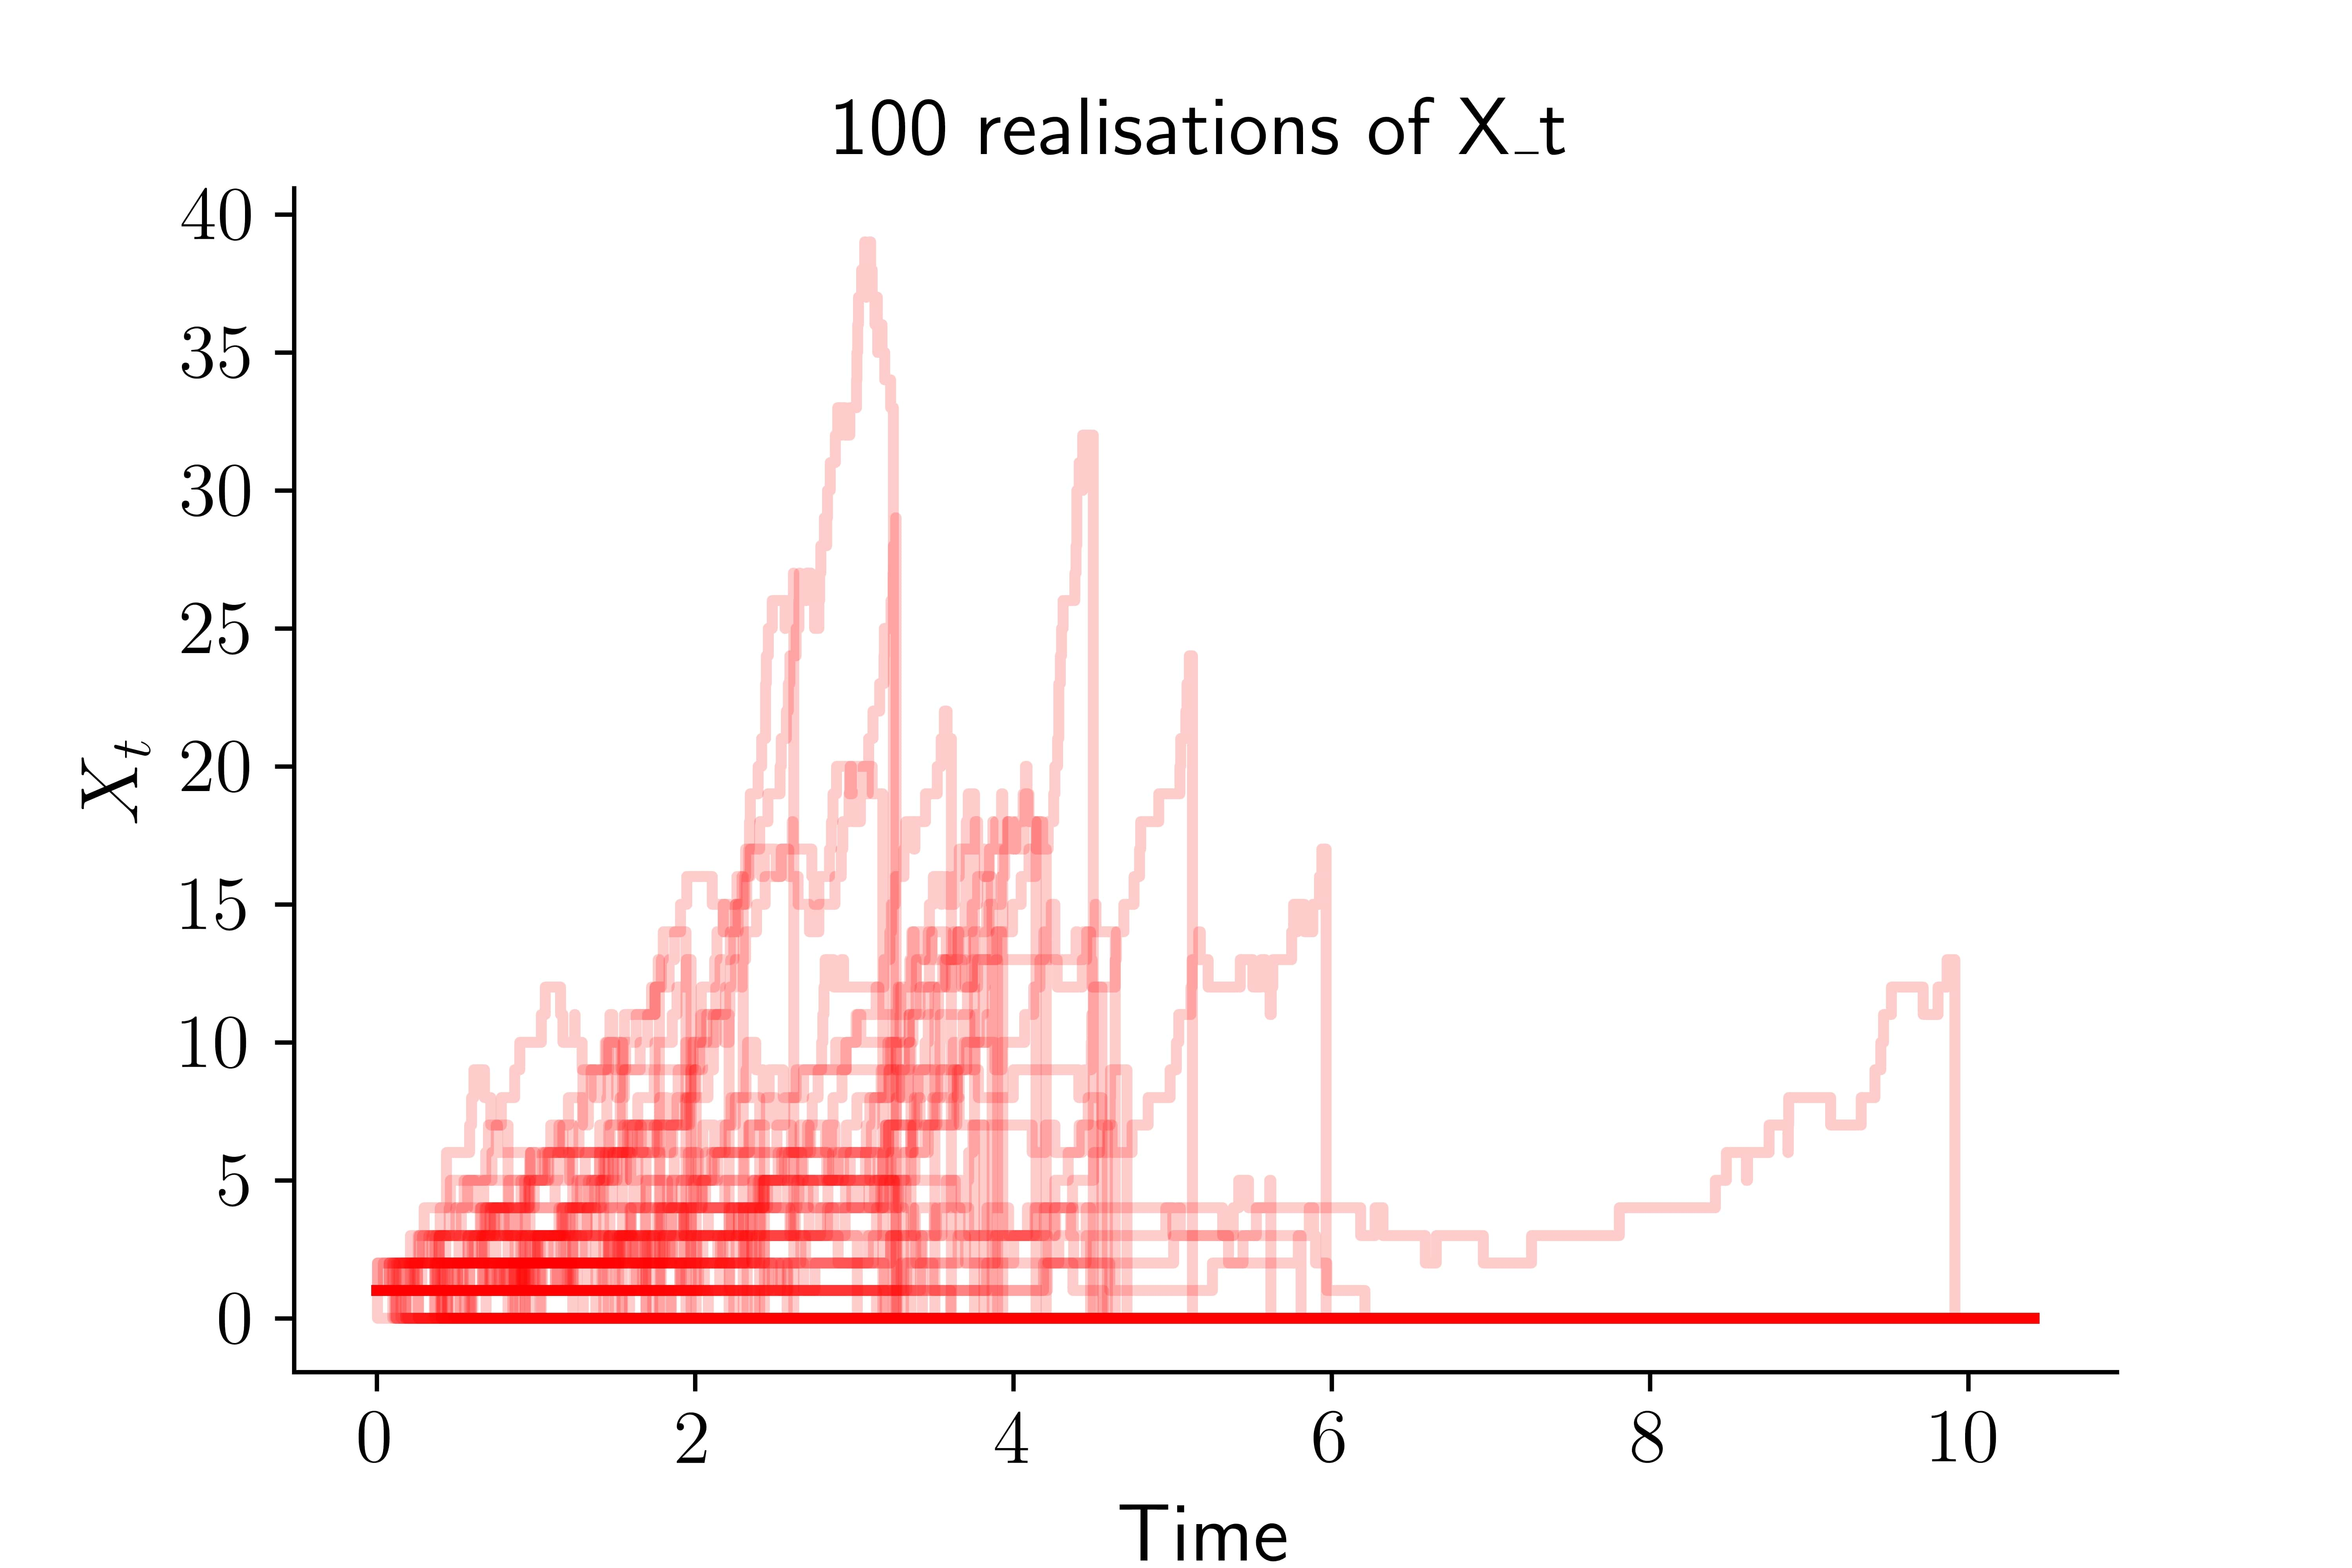
\includegraphics[width = 0.7\textwidth]{chapter4/IMG_ch4/BDRsimulations.jpg}
\caption{100 realisations of $\xt$ generated using the Gillespie algorithm. $\beta = 1$, $\mu = 0$, $\delta = 0.1$. }
\label{BDRsims}
\end{figure}


\subsection*{Choice of rupture state}


An alternative definition lists the ``catastrophe state'' as 0 instead of a $H$. And it would make some intuitive sense to arrange the process like this. After all, following rupture of an infected cell, there are subsequently 0 replicative units within it. But then, it also no longer exists. Ultimately, whether we ascribe the catastrophe state to 0 or $H$ is of no material significance to the dynamics. That is to say, the burst time and sizes observed are unchanged. But there is a distinction created in some of the formulas. These will be mentioned as we continue, but for our purposes, the catastrophe transition will be taken to the isolated state $H$. \par





\subsection*{Post catastrophe count}

For the context we are considering in which the catastrophe signifies the rupture of an infected cell, following this release, some count of infections units will enter the extracellular medium. This post rupture count, assuming no further dynamics, will be fixed by the final value of $\xt$ prior to catastrophe, and it will remain at that value for future time. We will refer to this post rupture count as $\wt$, itself a stochastic process. $\wt = 0$ for $t\leq\tau$, and $\wt = \xx_\tau$ thereafter for $t> \tau$. ($\tau$ being the time of cell rupture).\par
$\wt$ is included in the above definition as follows to describe the full stochastic process, ($\xt$, $\wt$).
\begin{align*}
\pr{\Delta \xt = 1, \Delta \wt = 0} &= \beta \xt \cdot \delt&&\text{(birth)}\\
\pr{\Delta \xt = -1, \Delta \wt = 0} &= \mu \xt  \cdot \delt&&\text{(death)}\\
\pr{\Delta \xt = 0, \Delta \wt = 0} &=1 -  (\beta+\mu+\delta) \xt  \cdot \delt&&\text{(no event)}\\
\pr{\xx_{t+\Delta t} = H, \ww_{t+\Delta t} = \xx_t} &=\delta \xt  \cdot \delt&&\text{(catastrophe)}
\end{align*}
(Using shorthand, $\Delta \xt = \xx_{t+\Delta t}  -  \xt$).


\begin{figure}[H]
\centering
\title{$\wt$}
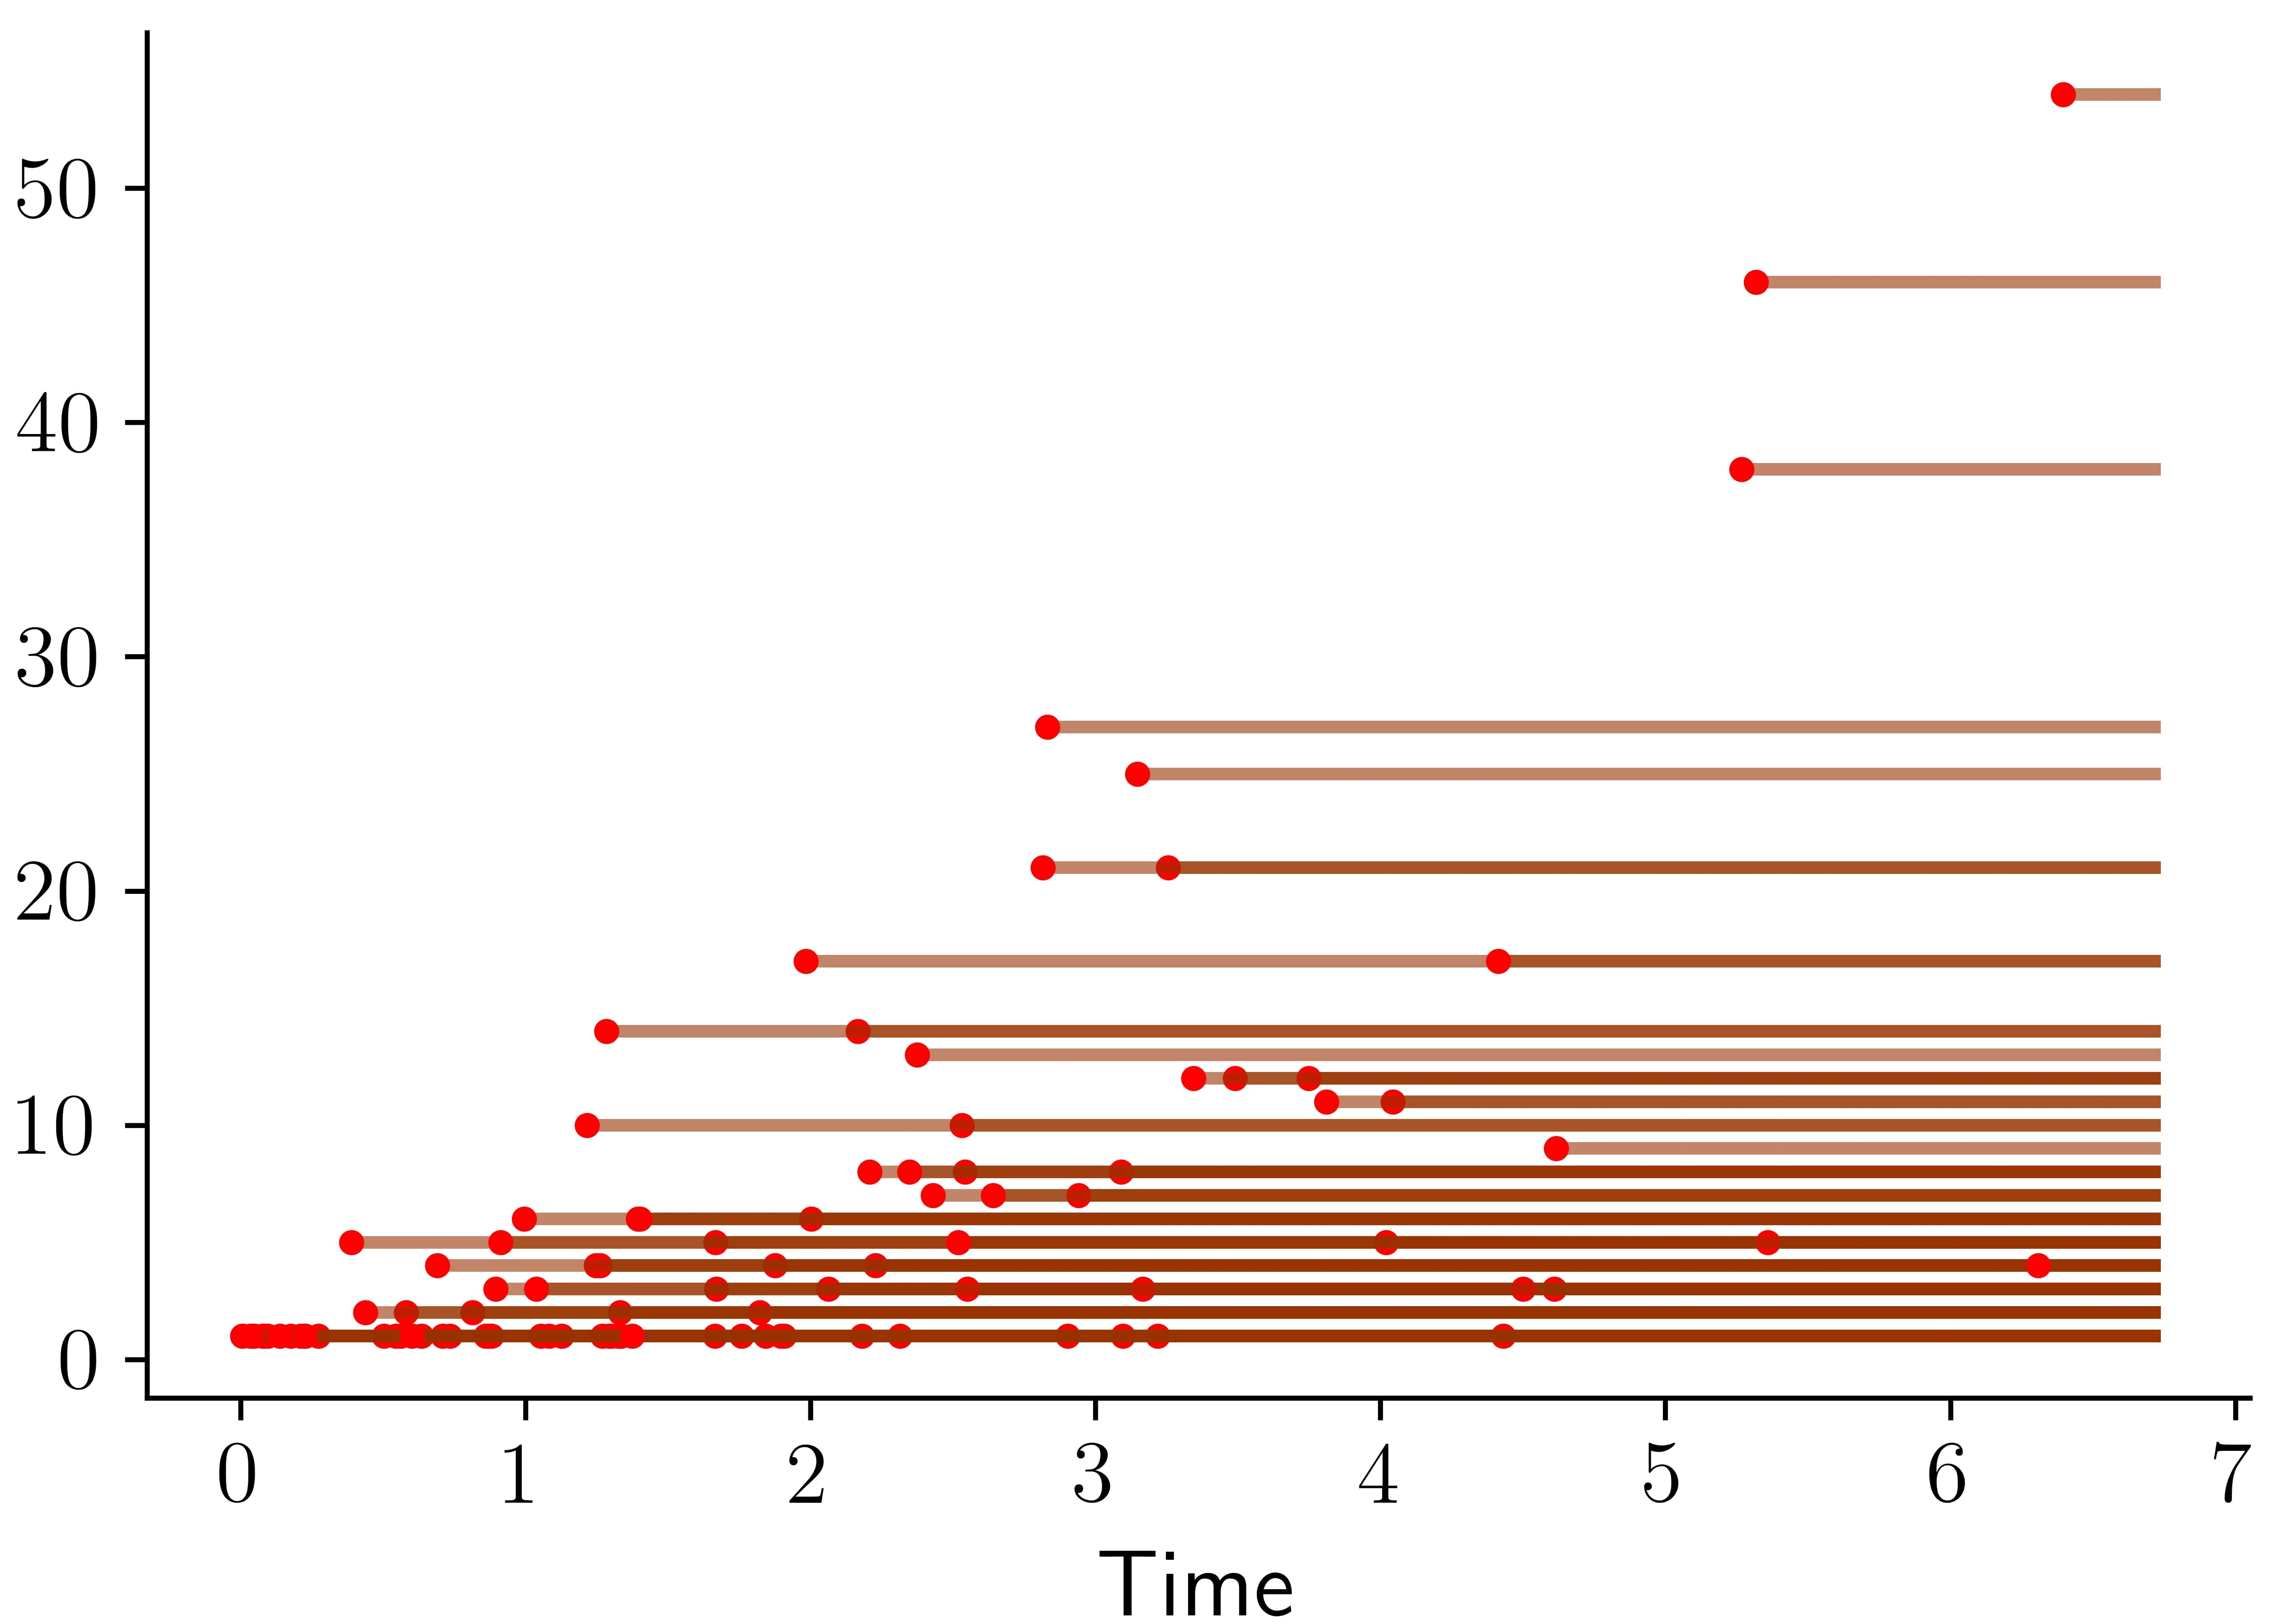
\includegraphics[width = 0.55\textwidth]{chapter4/IMG_ch4/BDRsimulationsY2.jpg}
\caption{100 realisations of $\wt$ generated using the Gillespie algorithm. $\beta = 1$, $\mu = 0$, $\delta = 0.1$. }
\label{BDRsims}
\end{figure}






















%%%%%%%%%%%%%%%%%%%%%%%%%%%%%%%%%%%%%%%%%%%%%%%%%%%%%%%%%%%%%%%%%%%%%%%%%%%%%%%%%%%%%%%%%%%%%%%%%%%%%%%%%%%

\section{Analytical quantities} 








To understand the dynamical properties of the BDC process, there are a handful of quantities for the focus of analysis.  



\subsection*{ ${I(t)}$, the non-catastrophe probability}

\vspace{3pt}
{\Large$$ I(t) = \pr{\xt \neq H|\; \xx_0 = 1}$$
$$\text{ \& }$$
$$\hat I(t) = \pr{\xt \notin \{0, H \}|\; \xx_0 = 1}$$}

\noindent
Given that the rupture state, $H$ is accessible from every non-zero state of the Markov process, eventual catastrophe is inevitable provided the process doesn't fixate by depletion to 0. Hence, either death or catastrophe is sure to happen at late time. $I(t)$ is the probability that the process has not experienced catastrophe prior to time $t$. 

 {\large $$I(t) = \frac{a(1-b) - b(1-a) \ee^{\lambda(a - b)t}}{(1-b) - (1-a) \ee^{\lambda(a - b)t}},$$}
 where 
$$a = \eta+\sqrt{\eta^2-\frac{\mu}{\lambda}}  \qquad  \text{ and } \qquad b =  \eta-\sqrt{\eta^2-\frac{\mu}{\lambda}},$$
with 
$$\eta = \frac{\lambda + \mu + \delta}{2\lambda}$$
This is the solution to a differential equation seen below. When $\mu>0$ and process death is possible.   It will tend down to the positive constant value, $b$, the likelihood of eventual  process death,
 $$\lrb{\lim_{t\to \infty}I(t) = \frac{-b(1-a)}{-(1-a)} = b}$$




\begin{figure}[H]
\xdef\mydelt{0.05}
\xdef\mybeta{1}
\xdef\mymu{0.2}
\begin{center}
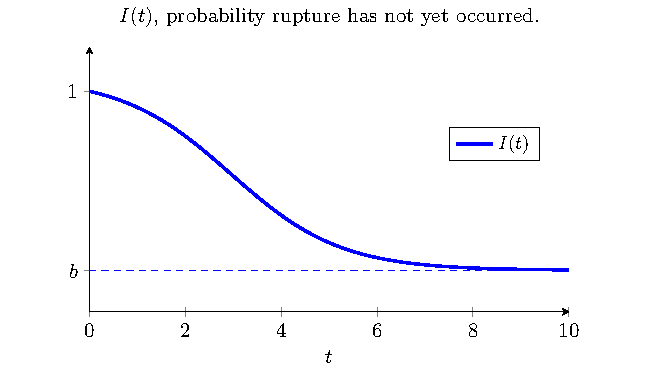
\includegraphics[width = 0.65\textwidth]{chapter4/IMG_ch4/I_of_t_1.pdf}
\end{center}
\caption{$I(t)$ plotted against time. Converges to $I_-$, representing the probability of eventual compartment recovery --- the birth death process dies out before rupture. $\beta=\mybeta$, $\mu=\mymu$, $\delta=\mydelt$}
\end{figure}



We can also consider the non-fixation probability, $\hat I(t)$, signifying the likelihood that at time $t$ the process has neither died, nor experienced catastrophe,
$$\hat I(t) = \pr{\xt \notin \{0, H \}|\; \xx_0 = 1}.$$ 
This will decline asymptotically to 0 signifying the eventual certainty of fixation one way or the other.  The solution is 

$$\hat I(t)  = \frac{2\eta}{1 - (1-2\eta)\ee^{2\eta\lambda t}},$$

$$\lim_{t\to \infty} \hat I(t) = 0.$$
The formulas for both $I(t)$ and $\hat I(t)$ are shown to result from their associated ODEs in the following section. Their form was first established by Kalin and Tavare in the 80s \cite{karlin1982linear}.



\begin{figure}[H]
\xdef\mydelt{0.05}
\xdef\mybeta{1}
\xdef\mymu{0.2}
\begin{center}
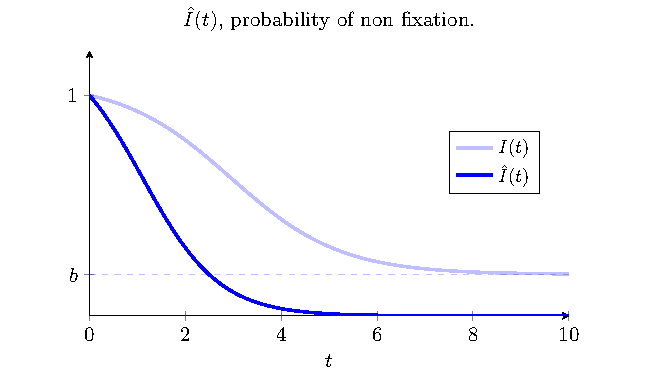
\includegraphics[width = 0.65\textwidth]{chapter4/IMG_ch4/I_of_t_2.pdf}
\end{center}
\caption{$\hat I(t)$ plotted against time. $\beta=\mybeta$, $\mu=\mymu$, $\delta=\mydelt$}
\end{figure}

\noindent
Suppose the process  begins with $k$ initial particles, $\xx_0 = k$. Each replicative unit gives rise to its own set of descendants, all behaving independently from one another. The likelihood through time that any one of those $k$ families will \textit{not} have led to catastrophe is $I(t)$. So it follows naturally, the probability that none of the $k$ families has led to the mass emigration is $\lrbs{I(t)}^k$;
$$  I_k(t) = \pr{\xt \neq H|\; \xx_0 = k} = \lrbs{I(t)}^k.$$
Likewise, when considering fixation more generally, 
$$\hat I_k(t) = \pr{\xt \notin \{0, H \}|\; \xx_0 = k}= \lrbs{\hat I(t)}^k.$$ 
(Is this correct?)










\subsection*{$J(t)$, replicative unit mean}

\vspace{3pt}
{\Large$$J(t) = \mean{\xt|\xx_0 = 1}$$}

\noindent
A given realisation of the process will rise and fall stochastically in steps for some time before ending up stuck either at 0 or, after catastrophe, at $H$. Following each of these fixation outcomes, the contribution of $\xt$ to the mean $J(t)$ is 0. So, supposing we observe 100 realisations, if at time $t=20$ all of them have have either died or undergone catastrophe, their sample mean would be 0 ($J_{\text{sample}}(20) = 0$).


From the initial condition, $\xx_0 = 1$, the process mean will go on to rise with realisations tending to increase, then fall as the likelihood of fixation grows asymptotically certain.

\begin{figure}[H]
\xdef\mydelt{0.05}
\xdef\mybeta{1}
\xdef\mymu{0.2}
\begin{center}
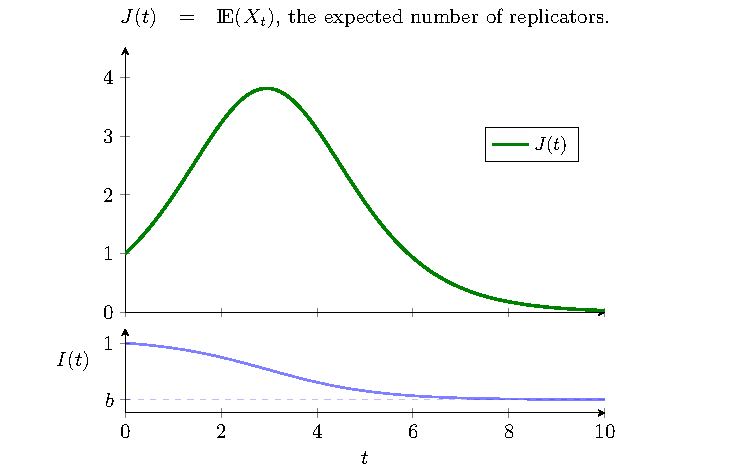
\includegraphics[width = 0.7\textwidth]{chapter4/IMG_ch4/J_of_t_1.pdf}
\end{center}
\caption{$J(t)$ plotted against time. $\beta=\mybeta$, $\mu=\mymu$, $\delta=\mydelt$}
\end{figure}

\noindent
It is given by the formula,

{\large$$J(t) = -\frac{\lambda(1-a)(1-b)(a-b)^2\ee^{\beta(a-b)t}}{\delta\big((1-b) - (1-a)\ee^{\lambda(a-b)t}\big)^2},$$}
which is obtained simply by differentiating $I(t)$ then multiplying by $-\delta^{-1}$. This follows from the equation $I' = -\delta J$ covered in more detail below.












\subsection*{$V(t)$, number of released units}

\vspace{3pt}
{\Large$$V(t) = \mean{\wt| \xx_0 = 1}$$}

\noindent
Over time, the process will either decline to 0, or transition to the catastrophe state, $H$. In which case, $\wt$ will be set at a geometrically distributed quantity seen in the final numeric value of $\xt$. $V(t)$, the expected post rupture count, incorporates all situations, whether $\wt$ is zero or not:

{\large $$V(t) = \frac{(\lambda - \mu)}{\delta}\big[1-I(t)\big] -J(t)+1. $$}
At late time, realisations which ended in both catastrophe, and death will constitute the value of $\lim_{t\to\infty} V(t) = V_{\infty}$.

$$V_{\infty} = \frac{(\lambda - \mu)}{\delta}\big[1-b\big]+1,$$
as $I\to b$ and $J \to 0$; when $\mu = 0$, 
$$V_{\infty} = \frac{\lambda }{\delta}+1.$$

For the case where death is included ($\mu>0$), the formula, $V_{\infty}$, takes into account eventualities in which the process did not attain catastrophe.
We may also extract the mean burst size proper by conditioning for cases which did experienced rupture, effectively discounting the dead realisations. This is done by dividing $V(t)$ by the likelihood of process catastrophe, $1-I(t)$. This is taken from the basic logic,
$$\mean{\wt} = \cancelto{0}{\mean{\wt | \text{no rupture}} I(t) }  + \mean{\wt | \text{rupture}} (1 - I(t)) $$
$$ \mean{\wt | \text{rupture}}  =  \frac{\mean{\wt}}{1 - I(t)},$$
$$\frac{V(t)}{1 - I(t)} $$
represents the expected burst size given catastrophe has taken place by time $t$. The ``overall'' burst size mean is seen in the late time value of this, incorporating all process realisations which experience rupture regardless of when:

\begin{align*}
\mean{\mathcal{K}} = \lim_{t\to \infty} \frac{V(t)}{1 - I(t)} &=  \frac{V_{\infty}}{1 - b} \\
&= \frac{\lambda-\mu}{\delta} + \frac{1}{1-b},
\end{align*}
(recalling that $b$ is the probability of ultimate process death). Notice the alignment $\mean{\mathcal{K}} = V_\infty$ when $\mu=0$. 



PLOT $\mean{\mathcal{K}}$ against $\delta$ for $\mu = 0$, $\lambda = 1$


	
\begin{figure}[H]
\begin{center}

\xdef\mydelt{0.05}
\xdef\mybeta{1}
\xdef\mysum{0.151}
\xdef\mymu{0.2}


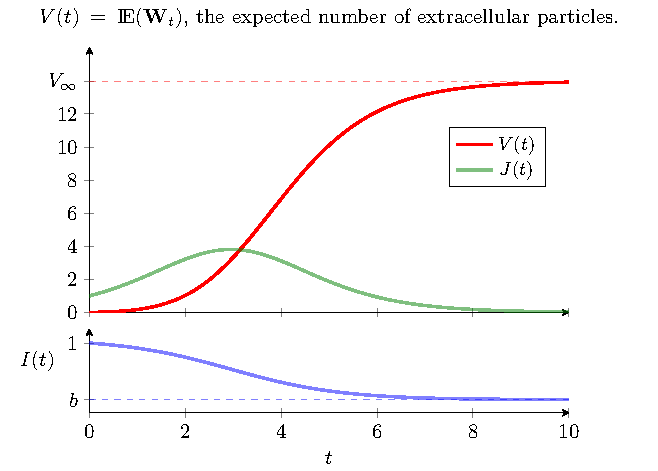
\includegraphics[width = 0.7\textwidth]{chapter4/IMG_ch4/V_of_t_1.pdf}

\end{center}
\caption{$V(t)$ plotted against time. $\beta=\mybeta$, $\mu=\mymu$, $\delta=\mydelt$.}
\end{figure}






\subsection*{$K(t)$, second moment of $\xt$}

\vspace{3pt}
{\Large$$K(t) = \mean{\xt^2| \xx_0 = 1}$$}

\noindent
We became interested in this quantity because it showed up in a term of the ODE describing change in $J(t)$:
$$\ddt{J} = (\lambda - \mu) J - \delta \mean{\xt^2}.$$
This final term results from the following reasoning. With rate $\delta \xt$, the value of $J(t)$ is reduced by $\xt$. So the expected deduction to $\xt$ by catastrophe over an infinitesimal duration is $\mean{ -\delta \xt^2 \delt}$. Hence, in deriving the above ODE, we find the contribution $-\delta \mean{\xt^2}$.




























%%%%%%%%%%%%%%%%%%%%%%%%%%%%%%%%%%%%%%%%%%%%%%%%%%%%%%%%%%%%%%%%%%%%%%%%%%%%%%%%%%%%%%%%%%%%%%%%%%%%%%%%%%%


\section{Derivation of equations and results}


\subsection{First equation}


{\large$$\ddt{I} = \mu - (\lambda + \mu + \delta) I + \lambda I^2$$}



Considering what may happen during an interval of duration $\delt$ after $t=0$, we can write down the equation,
$$I(0+\delt) = \mu \delt + [1 - (\beta + \mu + \delta)\delt] I(0) + \beta\delt {I(0)}^2 + o(\delt). $$
The single initial unit may die, divide, cause rupture, or do nothing at all; each possibility accounted for on the RHS, with the respective event-probabilities multiplied by the updated non-rupture likelihoods --- as if the process were beginning anew. In the case a rupture occurred, this value will obviously be 0; if a birth takes place, it assumes the value, $I_2(0)$. Which, as shown above is equivalent to ${I(0)}^2$. And because the model is homogeneous in time, the relation maintains applicability in subsequent intervals, $[t, t+\delt]$:
$$I(t+\delt) = \mu \delt + [1 - (\beta + \mu + \delta)\delt] I(t) + \beta\delt {I(t)}^2 + o(\delt). $$
Rearranging this yields, 
$$\frac{I(t+\delt) -I(t)}{\delt} = \mu - (\beta + \mu + \delta) I(t) + \beta {I(t)}^2 + \frac{o(\delt)}{\delt}.$$
Which, in the limit as $\delt\to 0$, becomes
\begin{equation}
\label{ddII}
\ddt{I} = \mu - (\beta + \mu + \delta) I + \beta {I}^2,
\end{equation}
a Ricatti equation with solution
\begin{equation}
\label{formI}
I(t) = \frac{I_+(1-I_-) - I_-(1-I_+) \ee^{\beta(I_+ - I_-)t}}{(1-I_-) - (1-I_+) \ee^{\beta(I_+ - I_-)t}}.
\end{equation}
Constants, $I_{\pm}$, given:
\begin{align*}
I_{\pm} = \eta \pm \sqrt{\eta^2 - \frac{\mu}{\beta}}\;, \hspace{20pt} \text{with}\hspace{20pt} \eta = \frac{\beta + \mu + \delta}{2\beta}.
\end{align*}

As an aside, it's worth mentioning that (\ref{ddII}) can be written in in terms of the constants, $I_{\pm}$:

\begin{equation}
\label{ddIIfact}
\ddt{I} =\beta\lrb{I-I_+}\lrb{I-I_+}.
\end{equation}



\noindent
Plotting $\dd I/\dd t$ against $I$ gives an intuitive picture of why $I(t)$ tends to $I_-$ at late time. 


\subsection{Alternative quantity to $I(t)$}
What if we consider the probability that the process has yet to reach the absorbing state of 0 --- by neither rupture, nor the birth-death process dying out? 
$$\hat I(t) = \pr{\xt \neq 0}.$$
When $\mu = 0$, this will be identical to $I(t)$.

The equivalent to equation (\ref{ddII}) is
\begin{equation}
\label{ddIIhat}
\ddt{\hat I} =  -(\beta + \mu + \delta)\hat I + \beta {\hat I}^2,
\end{equation}
as, during its derivation, in the case where the first unit dies, $\hat I(t)$ will become 0 rather than 1, so there is no $\mu$ term on the RHS.

(\ref{ddIIhat}) is solved by
$$\hat I(t) = \frac{\hat\eta}{1 - (1-\hat\eta)\ee^{\hat\eta\beta t}}, $$
with $\hat\eta = (\beta + \mu + \delta)/\beta$.











\section{Expected number of units,  $J(t) = \mean{\xt}$}

Individual realisations of the stochastic process, $\xt$, will vary greatly. When comparing a large number side by side, an increasing count will have collapsed to 0, as those remaining climb higher and higher. (assuming $\beta > \mu$). Despite this, we can quantify the expected (mean) value of the process over time --- call it $J(t)$: 
$$J(t) = \mean{\xt\;|\;\xx_0=1}.$$

\subsection{$J(t)$ as a formula in time}
A formula for $J(t)$ can be obtained with the following line of reasoning. 

Take the forward Kolmogorov equation describing $p_0(t) = \pr{\xt = 0}$.
$$\ddt{p_0} = \delta (1 p_1 + 2 p_2 + 3p_3  + \dots ) + \mu p_1$$
 On the RHS we see a sum of probabilities for the process being in a given state, multiplied by the relevant transition rates to 0. The end term, $\mu p_1$ is associated with death of the final living infectious particle. All of the others relate to catastrophe transitions, from every non-zero state, $i$, and with rates $\delta i$. These conveniently combine and make up the definition of $\mean{\xt}$. So we can write,
$$\ddt{p_0} = \delta J + \mu p_1.$$
Removing the $\mu p_1$ term, we are left with an equation describing the probability that $\xt$  equals $0$, \textit{and} it arrived there following a rupture event --- or, the probability that rupture has occurred. Call it $\hat p_0$. 
$$\ddt{\hat p_0} = \delta J.$$
Since $I(t)$ is the probability rupture has \textit{not} yet happened: $I(t) = 1-\hat p_0$. Hence,
\begin{equation}
\label{ddIJ}
\ddt{I} = -\delta J.
\end{equation}
(\ref{ddIJ}) can be rearranged ---
$$J = -\frac{1}{\delta}\ddt{I}$$
--- and solved for $J(t)$ by differentiating  (\ref{formI}), the formula for $I(t)$:
\begin{equation*}
J(t) = -\frac{\beta(1-I_+)(1-I_-)(I_+-I_-)^2\ee^{\beta(I_+-I_-)t}}{\delta\big((1-I_-) - (1-I_+)\ee^{\beta(I_+-I_-)t}\big)^2}
\end{equation*}







\subsection{Rate of change of $J$}

By looking to the list of possible events over a period $\delt$, we can write down the following relationship describing how $\mean{\xt}$ changes.
$$\mean{\xx_{t+\delt}} = \mean{\xt} + \mean{\xx_{t+\delt}-\xt};$$
the expected value of $\xx_{t+\delt}$ is what it was at time $t$, plus the expected change during the interval [$t$, $t+\delt$].
\begin{equation}
\label{ddJ}
\mean{\xx_{t+\delt}} = \mean{\xt} + \mean{\beta\delt\xt - \mu\delt\xt - \delta\delt\xt\cdot\xt}
\end{equation}
The final compenent, $- \delta\delt\xt\cdot\xt$, represents the probability that a rupture occurs during the interval, $\delta\delt\xt$, multiplied by the change to $\xt$ --- in this case: $-\xt$ (complete elimination).
Rearranging (\ref{ddJ}), we find 
$$\frac{\mean{\xx_{t+\delt}} - \mean{\xt}}{\delt} = \beta\mean{\xt} - \mu\mean{\xt} - \delta \mean{\xt^2}.$$
Which, evaluated in the limit, $\delt \to 0$, becomes
\begin{equation}
\label{ddJ2}
\ddt{J} = (\beta - \mu) J - \delta K(t),
\end{equation}
with
\begin{equation*}
K(t) = \mean{\xt^2}.
\end{equation*}


\subsection{Extracellular count, $V(t)$}

If we define a secondary process, $\yt$, as the number of units ``expelled'' following a rupture event in $\xt$, we can quantify the expected ``extracellular'' particle count through time. To clarify, $\yt$ will remain at 0 unless the associated process $\xt$ undergoes a catastrophe. With probability $1-I_-$, this will happen eventually, in which case $\yt$ will jump from 0 to the value of $\xt$ immediately prior to mass expulsion;
$$\pr{\yy_{t+\delt}-\yt = \xt,\; \xx_{t+\delt}-\xt=0} = \delta\xt\cdot\delt.$$



\noindent
By analogous reasoning that derived (\ref{ddJ2}), it is possible to state
\begin{equation}
\label{ddV}
\ddt{V} =  \delta K(t),
\end{equation}
where $V(t) = \mean{\yt}$.
And this can be solved for $V(t)$ in the following way. (\ref{ddJ2}) and (\ref{ddV}) combine to give,
$$\ddt{J} = (\beta - \mu) J - \ddt{V}.$$
With (\ref{ddIJ}), this can be rearranged into,
$$\ddt{V} = -\frac{(\beta - \mu)}{\delta}\ddt{I} - \ddt{J}.$$ 
Then, integrating:
$$V(t) = -\frac{(\beta - \mu)}{\delta}I(t) - J(t) + \text{const}.$$
And finally with initial conditions, $V(0) = 0$, and $J(0)=I(0)=1$,
\begin{equation*}
\label{Voft}
V(t) = \frac{(\beta - \mu)}{\delta}\big[1-I(t)\big] -J(t)+1.
\end{equation*}




\noindent
In late time, $V(t)$ will tend to
$$V_{\infty} =  \frac{(\beta - \mu)}{\delta}\big[1-I_-\big] +1,$$
which can be interpreted as the expected rupture size. 

When $\mu = 0$,
$$V_\infty = 1 +\frac{\beta}{\delta}.$$





\section{Variance and standard deviation of $\xt$ \& $\yt$}

To describe the variance of a random variable, it is standard to use the formula, 
\begin{equation*}
\text{Var}(\xt) = \mean{\xt^2} - \mean{\xt}^2.
\end{equation*}
And we can apply this to $\xt$ and $\yt$ to quantify the variability of intracellular and extracellular particles as functions of time. 

In each case, we will first require a formula for the expected value of the counts squared,  $\mean{\xt^2}$ and $\mean{\yt^2}$.






\subsection{Variance of $\xt$}

\subsubsection{Formula for $\mean{\xt^2}$ ($ = K(t)$)}

A formula for $K(t) = \mean{\xt^2}$ is derived in the following way. Taking the time derivative of equations,

 (\ref{ddIJ}): ${\rm d}I/{\rm d}t = -\delta J$, and, 
 
 (\ref{ddII}): ${\rm d}I/{\rm d}t = \mu - (\beta + \mu + \delta) I + \beta I^2$.

\begin{align}
\label{Kderev1}
\text{(\ref{ddIJ})}\to&&\ddt{J} = -\frac{1}{\delta}\frac{\dd^2 I}{\dd t^2}&&
\end{align}
\begin{align*}
\text{(\ref{ddII})}\to&& \frac{\dd^2 I}{\dd t^2} = -(\beta + \mu + \delta) \ddt{I} + 2\beta I \ddt{I}.&&
\end{align*}
The latter, with ${\rm d}I/{\rm d}t = -\delta J$, becomes
\begin{equation}
\label{Kderev2}
\frac{\dd^2 I}{\dd t^2} = (\beta + \mu + \delta)\beta J- 2\beta \delta I J.
\end{equation}
Comparing (\ref{Kderev2}) with (\ref{Kderev1}),
\begin{equation*}
%\label{Kderev3}
\ddt{J} = -(\beta + \mu + \delta) J + 2\beta I J;
\end{equation*}
then, this with (\ref{ddJ2}),
$$(\beta - \mu) J - \delta K = -(\beta + \mu + \delta) J + 2\beta I J.$$
Rearranging for $K(t)$,
\begin{equation}
\label{Kt1}
K(t) = \frac{2\beta}{\delta}\lrb{1+\frac{\delta}{2\beta} - I}J.
\end{equation}
Considering (\ref{ddIIfact}) and (\ref{ddIJ}), this may also be written as
\begin{equation}
\label{KtI}
K(I) = -\frac{2\beta^2}{\delta}\lrb{I-\kappa}\lrb{I-I_-}\lrb{I-I_+}.
\end{equation}
with,
$$\kappa = 1+\frac{\delta}{2\beta}.$$



\subsubsection{One standard deviation from the mean, $J(t)$}
With the expectation of $\xt^2$, (\ref{Kt1}), 
\begin{equation*}
K(t) = \frac{2\beta}{\delta}\lrb{\kappa- I}J,
\end{equation*}
we can write down the variance of $\xt$ using $\text{Var}(\xt) = \mean{\xt^2} - \mean{\xt}^2$:
\begin{align*}
\text{Var}(\xt) &= K(t) - {J(t)}^2\\
&= \frac{2\beta}{\delta}\lrb{\kappa - I}J - J^2.
\end{align*}
The standard deviation is then,
\begin{equation*}
\text{Std}(\xt) = \sqrt{\frac{2\beta}{\delta}\lrb{\kappa- I}J - J^2}.
\end{equation*}



\subsection{Variance of $\yt$}

We can likewise compute the variance of $\yt$ using $\text{Var}(\yt) = \mean{\yt^2} - \mean{\yt}^2$. To begin, we must find a formula for $\mean{\yt^2}$.


\subsubsection{Formula for $\mean{\yt^2}$}


Accounting for changes to $\yt^2$ over an infinitesimal time $\delt$,
$$\mean{\yy_{t+\delt}^2} = \mean{\yt^2} + \mean{\yy_{t+\delt}^2 - \yt^2},$$
we can derive the equation
\begin{equation}
\label{meanYt2}
\ddt{\mean{\yt^2}} = \delta \mean{\xt^3}.
\end{equation}
This might seem like a dead end as we have yet do come up with a description of $\mean{\xt^3}$. Though as it happens, the problem can be sidestepped by thinking about the rate of change of $K(t) = \mean{\xt^2}$. An equation for $\dd K/\dd t$ can be derived as follows. 
\begin{equation}
\label{meanysq1}
\mean{\xx_{t+\delt}^2} = \mean{\xt^2} + \mean{\xx_{t+\delt}^2 - \xt^2}
\end{equation}
Because of the quadratic, changes in $\xt^2$ require special attention (see table).
\begin{table}[ht]
\centering
\renewcommand{\arraystretch}{1.5} % Increase vertical padding
\setlength{\tabcolsep}{17pt} % Increase horizontal padding
\begin{tabular}{|>{\centering\arraybackslash}m{3cm}|>{\centering\arraybackslash}m{2cm}|>{\centering\arraybackslash}m{5cm}|}
\hline
Probability of occurrence& Change in $\xt$ & Change in $\xt^2$\\
\hline
\hline
$\beta \xt\delt$& 1 & $(\xt + 1)^2 - \xt^2 = 2\xt + 1$ \\
\hline
$\mu \xt\delt$ &-1 & $(\xt - 1)^2 - \xt^2 = -2\xt + 1$\\
\hline
$\delta \xt\delt$ & $-\xt$& $(\xt - \xt)^2 - \xt^2 = -\xt^2$ \\
\hline
\end{tabular}
\end{table}

\noindent
From the possibilities, it can be seen that
\begin{align*}\mean{\xx_{t+\delt}^2 - \xt^2} &={\rm I}\!{\rm E}\bigg[\beta \xt\delt\cdot(2\xt+1) + \mu \xt\delt\cdot(-2\xt+1) + \delta \xt\delt\cdot(-\xt)\bigg]\\
&=\bigg[ 2(\beta-\mu)\mean{\xt^2} + (\beta+\mu)\mean{\xt} - \delta\mean{\xt^3} \bigg]\delt
\end{align*}
Taking this with (\ref{meanysq1}), the following equation can be obtained in the $\downarrow \delt$ limit.
$$\ddt{\mean{\xt^2}} = 2(\beta-\mu)\mean{\xt^2} + (\beta + \mu)\mean{\xt} - \delta\mean{\xt^3};$$
it can also be written,
\begin{equation}
\label{ddK2}
\ddt{K} =2(\beta-\mu)K+ (\beta + \mu)J- \delta\mean{\xt^3}.
\end{equation}
With this, and equation (\ref{meanYt2}), we will see that it is possible to derive a formula for $\mean{\yt^2}$. 

Substituting into (\ref{ddK2}) with (\ref{meanYt2}), 
$$\ddt{K} =2(\beta-\mu)K+ (\beta + \mu)J- \ddt{\mean{\yt^2}}.$$
Then, using $J = \delta^{-1}\dd I/\dd t$ (\ref{ddIJ}), and $K = \delta^{-1} \dd V / \dd t$ (\ref{ddV}):
\begin{equation}
\ddt{\mean{\yt^2}} = 2\frac{(\beta-\mu)}{\delta}\ddt{V}+ \frac{(\beta + \mu)}{\delta}\ddt{I} - \ddt{K}.
\end{equation}
Which, with the initial conditions, $(I(0), K(0), V(0), \mean{\yy_0^2}) = (1,0,0,0)$, provides $\mean{\yt^2}$ by integration:
\begin{equation}
\label{meanEY2}
\mean{\yt^2} = 2\frac{\beta-\mu}{\delta} V + \frac{\beta+\mu}{\delta}I + K - \frac{\beta+\mu}{\delta}
\end{equation}


\subsubsection{One standard deviation from the mean, $V(t)$}

Using (\ref{meanEY2}), it is possible to write down a formula for the variance of $\yt$,
\begin{equation}
\label{VarY}
\text{Var}(\yt) = 2\frac{\beta-\mu}{\delta} V + \frac{\beta+\mu}{\delta}I + K - \frac{\beta+\mu}{\delta} - V^2
\end{equation}


























\section{Variable dependencies on $I(t)$}

It happens to be possible to write all of the formulas, $J(t)$, $\text{Var}(\xt)$, $V(t)$, $\text{Var}(\yt)$, as functions of the non-rupture probability $I(t)$. 


\subsection{Mean and variance of $\xt$}

Since $J = \delta^{-1}{\dd I}/{\dd t} $, and ${\dd I}/{\dd t} =  \beta (I - I_+)(I-I_-)$ (from (\ref{ddIJ})), we can write $J$ in terms of $I$:
\begin{equation}
\label{JI}
J(I) = -\frac{\beta}{\delta}  (I - I_+)(I-I_-).
\end{equation}
Combining this with (\ref{KtI}), we can also write $\text{Var}(\xt)$ as a function of $I(t)$,

\begin{align*}
\text{Var}(\xt) &= K(I) - {J(I)}^2\\
&=-\frac{2\beta^2}{\delta}\lrb{I-\kappa}\lrb{I-I_-}\lrb{I-I_+} - \lrb{\frac{\beta}{\delta}  (I - I_+)(I-I_-)}^2,
\end{align*}
$$\lrb{\kappa = 1+\frac{\delta}{2\beta}}.$$



\subsection{Mean and variance of $\yt$}

As we have defined $V(t)$ in terms of $I(t)$ and $J(t)$, it is likewise possible to use (\ref{JI}) to write $V(I)$, a function only of the non-rupture probability:
$$V(I) = \frac{\beta - \mu}{\delta}\lrb{1-I} + \frac{\beta}{\delta} (I - I_+)(I-I_-) + 1.$$
And given (\ref{VarY}), we can do the same for the variance of $\yt$:
$$\text{Var}(\yt) = 2\frac{\beta-\mu}{\delta} V(I) + \frac{\beta+\mu}{\delta}I + K(I) - \frac{\beta+\mu}{\delta} - {V(I)}^2;$$


\begin{multline*}
\text{Var}(\yt) = 2\frac{\beta - \mu}{\delta} \lrbs{ \frac{\beta - \mu}{\delta}\lrb{1-I} + \frac{\beta}{\delta} (I - I_+)(I-I_-) + 1} + \\
\frac{\beta+\mu}{\delta} I -\frac{2\beta^2}{\delta}\lrb{I-\kappa}\lrb{I-I_-}\lrb{I-I_+} - \frac{\beta + \mu}{\delta} - \\ \lrbs{\frac{\beta - \mu}{\delta}\lrb{1-I} + \frac{\beta}{\delta} (I - I_+)(I-I_-) + 1}^2.
\end{multline*}




































\section{Variance and standard deviation of $\xt$ \& $\yt$}

To describe the variance of a random variable, it is standard to use the formula, 
\begin{equation*}
\text{Var}(\xt) = \mean{\xt^2} - \mean{\xt}^2.
\end{equation*}
And we can apply this to $\xt$ and $\yt$ to quantify the variability of intracellular and extracellular particles as functions of time. 

In each case, we will first require a formula for the expected value of the counts squared,  $\mean{\xt^2}$ and $\mean{\yt^2}$.
These will be computed first.





\subsection{Variance of $\xt$}

\subsubsection{Formula for $\mean{\xt^2} = K(t)$}

$K(t) = \mean{\xt^2}$ is derived in the following way. Taking the time derivative of equations,

 (\ref{ddIJ}): ${\rm d}I/{\rm d}t = -\delta J$, and, 
 
 (\ref{ddII}): ${\rm d}I/{\rm d}t = \mu - (\beta + \mu + \delta) I + \beta I^2$.

\begin{align}
\label{Kderev1}
\text{(\ref{ddIJ})}\to&&\ddt{J} = -\frac{1}{\delta}\frac{\dd^2 I}{\dd t^2}&&
\end{align}
\begin{align*}
\text{(\ref{ddII})}\to&& \frac{\dd^2 I}{\dd t^2} = -(\beta + \mu + \delta) \ddt{I} + 2\beta I \ddt{I}.&&
\end{align*}
The latter, with ${\rm d}I/{\rm d}t = -\delta J$, becomes
\begin{equation}
\label{Kderev2}
\frac{\dd^2 I}{\dd t^2} = (\beta + \mu + \delta)\beta J- 2\beta \delta I J.
\end{equation}
Comparing (\ref{Kderev2}) with (\ref{Kderev1}),
\begin{equation*}
%\label{Kderev3}
\ddt{J} = -(\beta + \mu + \delta) J + 2\beta I J;
\end{equation*}
then, this with (\ref{ddJ2}),
$$(\beta - \mu) J - \delta K = -(\beta + \mu + \delta) J + 2\beta I J.$$
Rearranging for $K(t)$,
\begin{equation*}
K(t) = \frac{2\beta}{\delta}\lrb{1+\frac{\delta}{2\beta} - I}J
\end{equation*}



\subsubsection{One standard deviation from the mean, $J(t)$}
With the expectation of $\xt^2$,
\begin{equation*}
K(t) = \frac{2\beta}{\delta}\lrb{\kappa- I}J
\end{equation*}
$$\bigg( \kappa = 1+\frac{\delta}{2\beta}\bigg),$$
we can write down the variance of $\xt$ as,
\begin{align*}
\text{Var}(\xt) &= K(t) - {J(t)}^2\\
&= \frac{2\beta}{\delta}\lrb{\kappa - I}J - J^2.
\end{align*}
The standard deviation is then,
\begin{equation*}
\text{Std}(\xt) = \sqrt{\frac{2\beta}{\delta}\lrb{\kappa- I}J - J^2}.
\end{equation*}
























\section{Variable dependencies on $I(t)$}


\subsection{$J(I)$}

Since $J = \delta^{-1}{\dd I}/{\dd t} $, and ${\dd I}/{\dd t} =  \beta (I - I_+)(I-I_-)$ (from (\ref{ddIJ})), we can write $J$ in terms of $I$:

\begin{equation*}
J(I) = -\frac{\beta}{\delta}  (I - I_+)(I-I_-).
\end{equation*}


\subsection{$V(I)$}


Given this, $K$ can also be written as a function of $I$:
\begin{equation*}
K(I) = \frac{2\beta^2}{\delta^2}(I-k)(I - I_+)(I-I_-).
\end{equation*}
labelling $k = 1+ \delta/2\beta$. The same follows for $V$, and $\text{Var}(\xt)$:
\begin{equation*}
V(I) = \frac{\beta - \mu}{\delta}\lrbs{1-I} - J(I) + 1
\end{equation*}
\begin{equation*}
\text{Var}(\xt) = K(I) - J(I)^2
\end{equation*}




